\subsection{Testing testing...}
This is where the testing results go

some numbers for now: Transfers running since March, some 2.6 million transfers, 86.8 percent success
rate, over 2 PB of data so far. Approx. 7 percent of the rate CMS achieves globally.

The mesh...

% To create this graphic:
% 1) save your image as a 1024x1024 png/gif/bmp
% 2) convert to pdf (install ImageMagick, then 'convert FileIn.png FileOut.pdf')
\begin{figure}[htp]
\centering
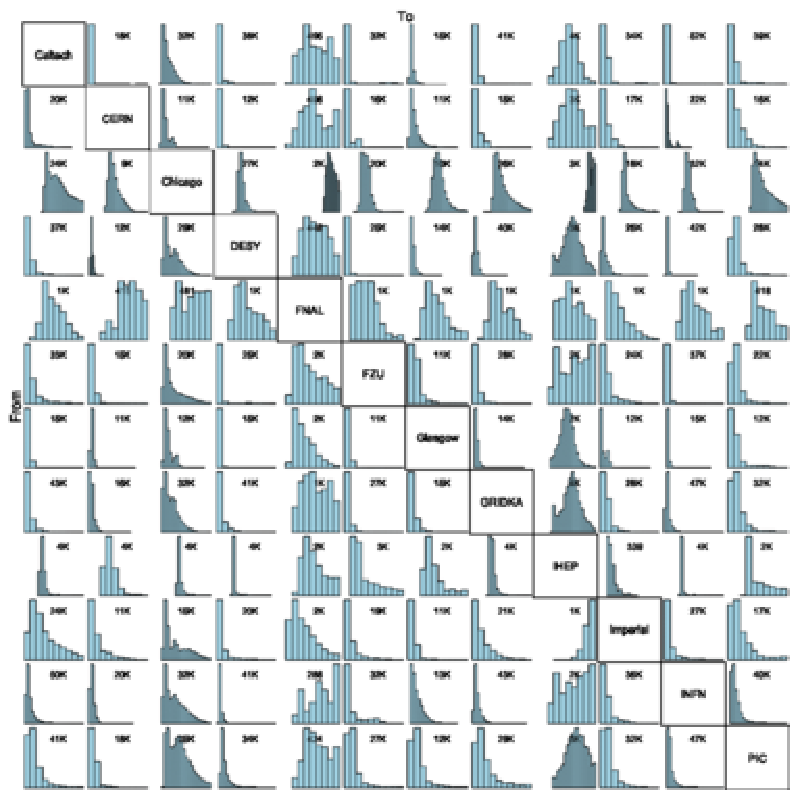
\includegraphics{full-mesh}
\caption{Transfer performance for the IPv6 testbed continuous transfers. A 1 GB file is transferred between each pair of sites, then deleted, then transferred again, continuously. The plots show the distribution of transfer duration times per site pair. The source site is named in the row, the destination site is named in the column. So the top-right plot shows transfers from Caltech to PIC, the bottom-left shows transfers fromPIC to Caltech. The x-axis is in seconds, from 0 to 500 for each plot. The number inset in each plot shows the approximate number of transfers between that site pair in that direction.}\label{fig:full-mesh}
\end{figure}

\subsection{Dual-stack at Imperial College HEP}
The WLCG site in the HEP group at Imperial College London (UKI-LT2-IC-HEP) has configured a large subset of its hosts to be dual-stack. 
This set up was achieved though a number of stages. Initially, the local campus network team enabled 
stateless address autoconfiguration (SLAAC) on the subnet routers servicing the grid hosts. All hosts got an IPv6 address via autoconfiguration. 
No subsequent problems were observed and no hosts required IPv6 to be turned off in order to continue normal operations. 
Next, AAAA records were added to core services such as mail and LDAP. The DNS servers had static IPv6 addresses added. 
The IPv6 DNS servers hostnames were added into resolve.conf on all hosts. AAAA and PTR records were added to the worker nodes and these were made to point at the SLAAC addresses. 
On relevant service hosts the IPv6 firewall was configured as appropriate. On hosts running a BDII service the IPv6 option was enabled explicitly 
(by setting BDII\_IPV6\_SUPPORT=yes in /etc/sysconfig/bdii). The site now runs DNS, SSH, NFS, EMI-2 and EMI-3 CREAM-CE's, 
ARC-CE (having once worked this is currently inoperational) and dCache (headnode, SRM component only) services. 
Additionally, all BDII services including top and site BDII's run in dual-stack mode. The Puppet configuration system and the local OS install system have been left IPv4-only.
